\section{Results}
\label{sec:results}

\section{Results for evolutionary approach 1}
\label{sec:results_1}

Like in Section \ref{sec:challenges} already mentioned unstable simulation results and non-reproducibility were encountered, which make it hard to interpret the results. Thus, good weights are interpreted mostly as weights with a high potential for a good reward.\\
The same evolutionary algorithm was tested with slightly different configurations concerning hyper-parameters. 
The best distances within every generation for different lengths of training periods and a population size within every generation of 30, were plotted with a logarithmic scale and can be seen in Fig. \ref{fig:results_1}. 

\begin{figure}[H]
	\centering
	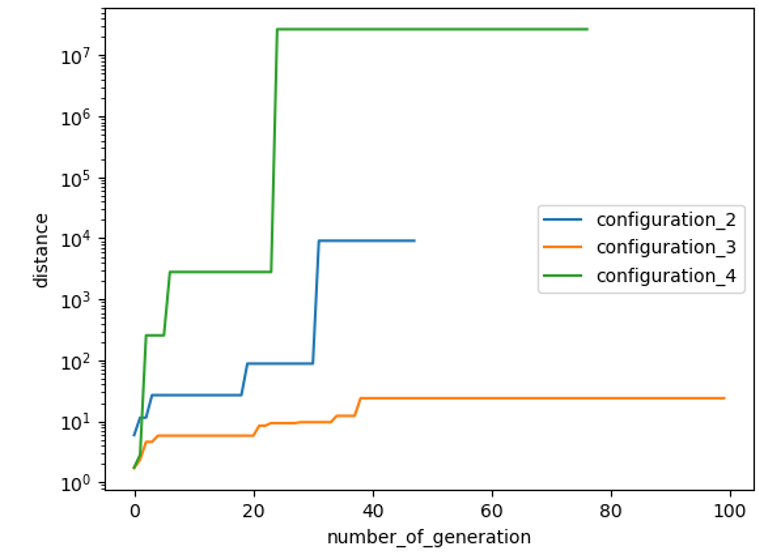
\includegraphics[width=3.3in]{img/results_1.png}
	\DeclareGraphicsExtensions.
	\caption{Results for different experiment configurations}
	\label{fig:results_1}
\end{figure}


The experiments were conducted with the following 4 different configurations:\\

\begin{itemize}
\item Configuration 1: 
\begin{itemize}
\item Output: 4 neurons to control 4 joints
\item fixed input of value 1
\item result was not plotted, overall best distance: 25 meters
\end{itemize}
\item Configuration 2: 
\begin{itemize}
\item Output: 7 neurons, 7 Joints 
\item Input: Position of Box (x, y, z) coordinates
\end{itemize}
\item Configuration 3: 
\begin{itemize}
\item Output: 7 neurons, 7 Joints 
\item Input: Position of Box rounded to second decimal place
\end{itemize}
\item Configuration 4: 
\begin{itemize}
\item Output: 7 neurons, 7 Joints and scaled output weights 
\item Input: Position of Box rounded to second decimal place
\end{itemize}
\end{itemize}

In general our algorithm was able to quickly find weights with high potential of great distances and even optimizing these weights as it would be desired.
But many of those distances were not reproducible due to instabilities of the distance calculation of the platform or bugs which occurred in the physics simulation. Therefore the best distances often were only rarely reproducible. Nevertheless the algorithm still performed well on the given prerequisites.

\section{Results for evolutionary approach 2}
The second evolutionary approach was only conducted once with the following configuration:
\begin{itemize}
	\item Output: 7 neurons, 7 Joints and scaled output weights 
	\item Input: fixed input of value 1
\end{itemize}
\begin{figure}[H]
	\centering
	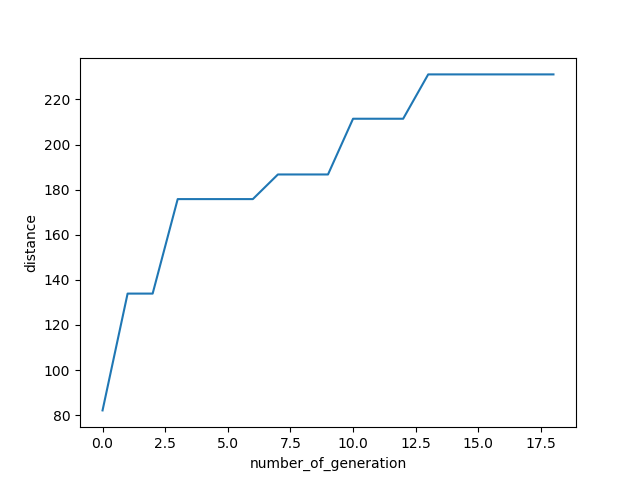
\includegraphics[width=3.3in]{img/approach2.png}
	\DeclareGraphicsExtensions.
	\caption{Results of the second evolutionary strategy}
	\label{fig:results_2}
\end{figure}
We chose a population size of 20 and ran the experiment for 20 generations. The training achieved a high distance early in the second generation which was due to the unstable physics simulation of the robot arm. Nevertheless the network was able to reproduce this error several times in the following generations. The results can be seen in Fig. \ref{fig:results_2}.

\section{Conclusion}
A brief introduction into genetic algorithms, reinforcement learning and spiking neural networks was given and the reason for the algorithm choice of the given task was elaborated in this paper. The different approaches were described theoretically and problems were discussed. We confirmed that the proposed method learns a set of weights with high potential in acceptable time. Finally the results are given for each of the approaches and its sub-configurations and an interpretation of those was given.
Future research can be done on other learning strategies or optimizing the hyper-parameters for the evolutionary strategy 2, elaborated in Section \ref{sec:strategie_2}.